\documentclass[landscape, 11pt]{article}

\usepackage{assign}

\setcoursetitle{CS335: Compiler Design}
\setauthname{Prann Bansal, Manish Kumar Bera, Gurpreet Singh}
\setauthroll{150259}
\setheaddate{21 January, 2018}
\setassigncode{0}

\begin{document}
\makeheader

\begin{qsection}{Team Members} \vspace{5mm}

	\begin{center}
		\begin{tabular}[h!]{lC{3.5cm}l}
			\hline
			\bt{Names}			&	\bt{Roll Numbers}	&	\bt{Email} 			\\
			\hline
			Manish Kumar Bera	&	150381				&	mkbera@iitk.ac.in	\\
			Prann Bansal		&	150510				&	prann@iitk.ac.in	\\
			Gurpreet Singh		&	150259				&	guggu@iitk.ac.in	\\
			\hline
		\end{tabular}
	\end{center}

\end{qsection}

\begin{qsection}{T-Diagram}

	\begin{figure}[h!]
		\centering
		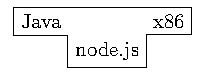
\includegraphics[height=60px]{includes/t-diagram.pdf}
		\caption{T-Diagram for the proposed compiler}
		\label{fig:t-diagram}
	\end{figure}

	The T-Diagram for the proposed compiler is given in Figure \ref{fig:t-diagram}. We aim to build a compiler for a subset of the Java programming language, compiled to the assembly language MIPS, on a Node.js platform.

\end{qsection}

\begin{qsection}{BNF}

	Below, we provide the subset of the Java BNF obtained from ---
	\ct{\href{https://users-cs.au.dk/amoeller/dRegAut/JavaBNF.html}{https://users-cs.au.dk/amoeller/dRegAut/JavaBNF.html}} \br

	\begin{enumerate}[label=\bt{\theenumi.}]
		\tt
		\ditem[Programs.]

			\begin{longtable}{R{7cm} c L{15cm}}
				\bt{LHS}									&					&	\bt{RHS} \\
				<compilation unit>							&	$\colon\colon=$	&	<import declarations>? <type declarations>?
			\end{longtable}

		\ditem[Declarations.]

			\begin{longtable}{R{7cm} c L{15cm}}
				\bt{LHS}									&					&	\bt{RHS} \\
				<import declarations>						&	$\colon\colon=$	&	<import declaration> | <import declarations> <import declaration>
				\\
				<import declaration>						&	$\colon\colon=$	&	<single type import declaration> | <type import on demand declaration>
				\\
				<single type import declaration>			&	$\colon\colon=$	&	import <type name> ;
				\\
				<type declarations>							&	$\colon\colon=$	&	<type declaration> | <type declarations> <type declaration>
				\\
				<type declaration>							&	$\colon\colon=$	&	<class declaration> | ;
				\\
				<class declaration>							&	$\colon\colon=$	&	<class modifiers>? class <identifier> <super>? <class body>
				\\
				<class modifiers>							&	$\colon\colon=$	&	<class modifier> | <class modifiers> <class modifier>
				\\
				<class modifier>							&	$\colon\colon=$	&	public
				\\
				<super>										&	$\colon\colon=$	&	extends <class type>
				\\
				<class body>								&	$\colon\colon=$	&	{ <class body declarations>? }
				\\
				<class body declarations>					&	$\colon\colon=$	&	<class body declaration> | <class body declarations> <class body declaration>
				\\
				<class body declaration>					&	$\colon\colon=$	&	<class member declaration> | <static initializer> | <constructor declaration>
				\\
				<class member declaration>					&	$\colon\colon=$	&	<field declaration> | <method declaration>
				\\
				<static initializer>						&	$\colon\colon=$	&	static <block>
				\\
				<constructor declaration>					&	$\colon\colon=$	&	<constructor modifiers>? <constructor declarator> <constructor body>
				\\
				<constructor modifiers>						&	$\colon\colon=$	&	<constructor modifier> | <constructor modifiers> <constructor modifier>
				\\
				<constructor modifier>						&	$\colon\colon=$	&	public
				\\
				<constructor declarator>					&	$\colon\colon=$	&	<type name> ( <formal parameter list>? )
				\\
				<formal parameter list>						&	$\colon\colon=$	&	<formal parameter> | <formal parameter list> , <formal parameter>
				\\
				<formal parameter>							&	$\colon\colon=$	&	<type> <variable declarator id>
				\\
				<constructor body>							&	$\colon\colon=$	&	{ <explicit constructor invocation>? <block statements>? }
				\\
				<explicit constructor invocation>			&	$\colon\colon=$	&	this ( <argument list>? ) | super ( <argument list>? )
				\\
				<field declaration>							&	$\colon\colon=$	&	<field modifiers>? <type> <variable declarators> ;
				\\
				<field modifiers>							&	$\colon\colon=$	&	<field modifier> | <field modifiers> <field modifier>
				\\
				<field modifier>							&	$\colon\colon=$	&	public | static
				\\
				<variable declarators>						&	$\colon\colon=$	&	<variable declarator> | <variable declarators> , <variable declarator>
				\\
				<variable declarator>						&	$\colon\colon=$	&	<variable declarator id> | <variable declarator id> = <variable initializer>
				\\
				<variable declarator id>					&	$\colon\colon=$	&	<identifier> | <variable declarator id> [ ]
				\\
				<variable initializer>						&	$\colon\colon=$	&	<expression> | <array initializer>
				\\
				<method declaration>						&	$\colon\colon=$	&	<method header> <method body>
				\\
				<method header>								&	$\colon\colon=$	&	<method modifiers>? <result type> <method declarator>
				\\
				<result type>								&	$\colon\colon=$	&	<type> | void
				\\
				<method modifiers>							&	$\colon\colon=$	&	<method modifier> | <method modifiers> <method modifier>
				\\
				<method modifier>							&	$\colon\colon=$	&	public | static
				\\
				<method declarator>							&	$\colon\colon=$	&	<identifier> ( <formal parameter list>? )
				\\
				<method body>								&	$\colon\colon=$	&	<block> | ;
				\\
				<constant declaration>						&	$\colon\colon=$	&	<constant modifiers> <type> <variable declarator>
				\\
				<constant modifiers>						&	$\colon\colon=$	&	public | static
				\\
				<array initializer>							&	$\colon\colon=$	&	{ <variable initializers>? , ? }
				\\
				<variable initializers>						&	$\colon\colon=$	&	<variable initializer> | <variable initializers> , <variable initializer>
				\\
				<variable initializer>						&	$\colon\colon=$	&	<expression> | <array initializer>
			\end{longtable}

		\ditem[Types.]

			\begin{longtable}{R{7cm} c L{15cm}}
				\bt{LHS}									&					&	\bt{RHS} \\
				<block>										&	$\colon\colon=$	&	{ <block statements>? }
				\\
				<block statements>							&	$\colon\colon=$	&	<block statement> | <block statements> <block statement>
				\\
				<block statement>							&	$\colon\colon=$	&	<local variable declaration statement> | <statement>
				\\
				<local variable declaration statement>		&	$\colon\colon=$	&	<local variable declaration> ;
				\\
				<local variable declaration>				&	$\colon\colon=$	&	<type> <variable declarators>
				\\
				<statement>									&	$\colon\colon=$	&	<statement without trailing substatement> | <if then statement> | <if then else statement> | <while statement> | <for statement>
				\\
				<statement no short if>						&	$\colon\colon=$	&	<statement without trailing substatement> | <if then else statement no short if> | <while statement no short if> | <for statement no short if>
				\\
				<statement without trailing substatement>	&	$\colon\colon=$	&	<block> | <empty statement> | <expression statement> | <switch statement> | <do statement> | <break statement> | <continue statement> | <return statement>
				\\
				<empty statement>							&	$\colon\colon=$	&	;
				\\
				<expression statement>						&	$\colon\colon=$	&	<statement expression> ;
				\\
				<statement expression>						&	$\colon\colon=$	&	<assignment> | <preincrement expression> | <postincrement expression> | <predecrement expression> | <postdecrement expression> | <method invocation> | <class instance creation expression>
				\\
				<if then statement>							&	$\colon\colon=$	&	if ( <expression> ) <statement>
				\\
				<if then else statement>					&	$\colon\colon=$	&	if ( <expression> ) <statement no short if> else <statement>
				\\
				<if then else statement no short if>		&	$\colon\colon=$	&	if ( <expression> ) <statement no short if> else <statement no short if>
				\\
				<switch statement>							&	$\colon\colon=$	&	switch ( <expression> ) <switch block>
				\\
				<switch block>								&	$\colon\colon=$	&	{ <switch block statement groups>? <switch labels>? }
				\\
				<switch block statement groups>				&	$\colon\colon=$	&	<switch block statement group> | <switch block statement groups> <switch block statement group>
				\\
				<switch block statement group>				&	$\colon\colon=$	&	<switch labels> <block statements>
				\\
				<switch labels>								&	$\colon\colon=$	&	<switch label> | <switch labels> <switch label>
				\\
				<switch label>								&	$\colon\colon=$	&	case <constant expression> : | default :
				\\
				<while statement>							&	$\colon\colon=$	&	while ( <expression> ) <statement>
				\\
				<while statement no short if>				&	$\colon\colon=$	&	while ( <expression> ) <statement no short if>
				\\
				<do statement>								&	$\colon\colon=$	&	do <statement> while ( <expression> ) ;
				\\
				<for statement>								&	$\colon\colon=$	&	for ( <for init>? ; <expression>? ; <for update>? ) <statement>
				\\
				<for statement no short if>					&	$\colon\colon=$	&	for ( <for init>? ; <expression>? ; <for update>? ) <statement no short if>
				\\
				<for init>									&	$\colon\colon=$	&	<statement expression list> | <local variable declaration>
				\\
				<for update>								&	$\colon\colon=$	&	<statement expression list>
				\\
				<statement expression list>					&	$\colon\colon=$	&	<statement expression> | <statement expression list> , <statement expression>
				\\
				<break statement>							&	$\colon\colon=$	&	break ;
				\\
				<continue statement>						&	$\colon\colon=$	&	continue ;
				\\
				<return statement>							&	$\colon\colon=$	&	return <expression>? ;
			\end{longtable}

		\ditem[Blocks and Commands.]

			\begin{longtable}{R{7cm} c L{15cm}}
				\bt{LHS}									&					&	\bt{RHS} \\
				<constant expression>						&	$\colon\colon=$	&	<expression>
				\\
				<expression>								&	$\colon\colon=$	&	<assignment expression>
				\\
				<assignment expression>						&	$\colon\colon=$	&	<conditional expression> | <assignment>
				\\
				<assignment>								&	$\colon\colon=$	&	<left hand side> <assignment operator> <assignment expression>
				\\
				<left hand side>							&	$\colon\colon=$	&	<expression name> | <field access> | <array access>
				\\
				<assignment operator>						&	$\colon\colon=$	&	= | *= | /= | \%= | += | -= | <<= | >>= | \&= | $\wedge$= | |=
				\\
				<conditional expression>					&	$\colon\colon=$	&	<conditional or expression> | <conditional or expression> ? <expression> : <conditional expression>
				\\
				<conditional or expression>					&	$\colon\colon=$	&	<conditional and expression> | <conditional or expression> || <conditional and expression>
				\\
				<conditional and expression>				&	$\colon\colon=$	&	<inclusive or expression> | <conditional and expression> \&\& <inclusive or expression>
				\\
				<inclusive or expression>					&	$\colon\colon=$	&	<exclusive or expression> | <inclusive or expression> \#| <exclusive or expression>
				\\
				<exclusive or expression>					&	$\colon\colon=$	&	<and expression> | <exclusive or expression> $\wedge$ <and expression>
				\\
				<and expression>							&	$\colon\colon=$	&	<equality expression> | <and expression> \& <equality expression>
				\\
				<equality expression>						&	$\colon\colon=$	&	<relational expression> | <equality expression> == <relational expression> | <equality expression> != <relational expression>
				\\
				<relational expression>						&	$\colon\colon=$	&	<shift expression> | <relational expression> < <shift expression> | <relational expression> > <shift expression> | <relational expression> <= <shift expression> | <relational expression> >= <shift expression> | <relational expression> instanceof <reference type>
				\\
				<shift expression>							&	$\colon\colon=$	&	<additive expression> | <shift expression> << <additive expression> | <shift expression> >> <additive expression>
				\\
				<additive expression>						&	$\colon\colon=$	&	<multiplicative expression> | <additive expression> + <multiplicative expression> | <additive expression> - <multiplicative expression>
				\\
				<multiplicative expression>					&	$\colon\colon=$	&	<unary expression> | <multiplicative expression> * <unary expression> | <multiplicative expression> / <unary expression> | <multiplicative expression> \% <unary expression>
				\\
				<cast expression>							&	$\colon\colon=$	&	( <primitive type> ) <unary expression> | ( <reference type> ) <unary expression not plus minus>
				\\
				<unary expression>							&	$\colon\colon=$	&	<preincrement expression> | <predecrement expression> | + <unary expression> | - <unary expression> | <unary expression not plus minus>
				\\
				<predecrement expression>					&	$\colon\colon=$	&	-- <unary expression>
				\\
				<preincrement expression>					&	$\colon\colon=$	&	++ <unary expression>
				\\
				<unary expression not plus minus>			&	$\colon\colon=$	&	<postfix expression> | ~ <unary expression> | ! <unary expression> | <cast expression>
				\\
				<postdecrement expression>					&	$\colon\colon=$	&	<postfix expression> --
				\\
				<postincrement expression>					&	$\colon\colon=$	&	<postfix expression> ++
				\\
				<postfix expression>						&	$\colon\colon=$	&	<primary> | <expression name> | <postincrement expression> | <postdecrement expression>
				\\
				<method invocation>							&	$\colon\colon=$	&	<method name> ( <argument list>? ) | <primary> . <identifier> ( <argument list>? ) | super . <identifier> ( <argument list>? )
				\\
				<field access>								&	$\colon\colon=$	&	<primary> . <identifier> | super . <identifier>
				\\
				<primary>									&	$\colon\colon=$	&	<primary no new array> | <array creation expression>
				\\
				<primary no new array>						&	$\colon\colon=$	&	<literal> | this | ( <expression> ) | <class instance creation expression> | <field access> | <method invocation> | <array access>
				\\
				<class instance creation expression>		&	$\colon\colon=$	&	new <class type> ( <argument list>? )
				\\
				<argument list>								&	$\colon\colon=$	&	<expression> | <argument list> , <expression>
				\\
				<array creation expression>					&	$\colon\colon=$	&	new <primitive type> <dim exprs> <dims>? | new <class or interface type> <dim exprs> <dims>?
				\\
				<dim exprs>									&	$\colon\colon=$	&	<dim expr> | <dim exprs> <dim expr>
				\\
				<dim expr>									&	$\colon\colon=$	&	[ <expression> ]
				\\
				<dims>										&	$\colon\colon=$	&	[ ] | <dims> [ ]
				\\
				<array access>								&	$\colon\colon=$	&	<expression name> [ <expression> ] | <primary no new array> [ <expression>]
			\end{longtable}

		\ditem[Expressions.]

			\begin{longtable}{R{7cm} c L{15cm}}
				\bt{LHS}									&					&	\bt{RHS} \\
				<constant expression>						&	$\colon\colon=$	&	<expression>
				\\
				<expression>								&	$\colon\colon=$	&	<assignment expression>
				\\
				<assignment expression>						&	$\colon\colon=$	&	<conditional expression> | <assignment>
				\\
				<assignment>								&	$\colon\colon=$	&	<left hand side> <assignment operator> <assignment expression>
				\\
				<left hand side>							&	$\colon\colon=$	&	<expression name> | <field access> | <array access>
				\\
				<assignment operator>						&	$\colon\colon=$ &	= | *= | /= | \%= | += | -= | <<= | >>= | \&= | $\wedge$= | |=
				\\
				<conditional expression>					&	$\colon\colon=$	&	<conditional or expression> | <conditional or expression> ? <expression> : <conditional expression>
				\\
				<conditional or expression>					&	$\colon\colon=$	&	<conditional and expression> | <conditional or expression> || <conditional and expression>
				\\
				<conditional and expression>				&	$\colon\colon=$ &	<inclusive or expression> | <conditional and expression> \&\& <inclusive or expression>
				\\
				<inclusive or expression>					&	$\colon\colon=$	&	<exclusive or expression> | <inclusive or expression> \ut{|} <exclusive or expression>
				\\
				<exclusive or expression>					&	$\colon\colon=$ &	<and expression> | <exclusive or expression> $\wedge$ <and expression>
				\\
				<and expression>							&	$\colon\colon=$	&	<equality expression> | <and expression> \& <equality expression>
				\\
				<equality expression>						&	$\colon\colon=$	&	<relational expression> | <equality expression> == <relational expression> | <equality expression> != <relational expression>
				\\
				<relational expression>						&	$\colon\colon=$	&	<shift expression> | <relational expression> < <shift expression> | <relational expression> > <shift expression> | <relational expression> <= <shift expression> | <relational expression> >= <shift expression> | <relational expression> instanceof <reference type>
				\\
				<shift expression>							&	$\colon\colon=$	&	<additive expression> | <shift expression> << <additive expression> | <shift expression> >> <additive expression>
				\\
				<additive expression>						&	$\colon\colon=$	&	<multiplicative expression> | <additive expression> + <multiplicative expression> | <additive expression> - <multiplicative expression>
				\\
				<multiplicative expression>					&	$\colon\colon=$	&	<unary expression> | <multiplicative expression> * <unary expression> | <multiplicative expression> / <unary expression> | <multiplicative expression> \% <unary expression>
				\\
				<cast expression>							&	$\colon\colon=$	&	( <primitive type> ) <unary expression> | ( <reference type> ) <unary expression not plus minus>
				\\
				<unary expression>							&	$\colon\colon=$	&	<preincrement expression> | <predecrement expression> | + <unary expression> | - <unary expression> | <unary expression not plus minus>
				\\
				<predecrement expression>					&	$\colon\colon=$	&	-- <unary expression>
				\\
				<preincrement expression>					&	$\colon\colon=$	&	++ <unary expression>
				\\
				<unary expression not plus minus>			&	$\colon\colon=$	&	<postfix expression> | ~ <unary expression> | ! <unary expression> | <cast expression>
				\\
				<postdecrement expression>					&	$\colon\colon=$	&	<postfix expression> --
				\\
				<postincrement expression>					&	$\colon\colon=$	&	<postfix expression> ++
				\\
				<postfix expression>						&	$\colon\colon=$	&	<primary> | <expression name> | <postincrement expression> | <postdecrement expression>
				\\
				<method invocation>							&	$\colon\colon=$	&	<method name> ( <argument list>? ) | <primary> . <identifier> ( <argument list>? ) | super . <identifier> ( <argument list>? )
				\\
				<field access>								&	$\colon\colon=$	&	<primary> . <identifier> | super . <identifier>
				\\
				<primary>									&	$\colon\colon=$	&	<primary no new array> | <array creation expression>
				\\
				<primary no new array>						&	$\colon\colon=$	&	<literal> | this | ( <expression> ) | <class instance creation expression> | <field access> | <method invocation> | <array access>
				\\
				<class instance creation expression>		&	$\colon\colon=$	&	new <class type> ( <argument list>? )
				\\
				<argument list>								&	$\colon\colon=$	&	<expression> | <argument list> , <expression>
				\\
				<array creation expression>					&	$\colon\colon=$	&	new <primitive type> <dim exprs> <dims>? | new <class or interface type> <dim exprs> <dims>?
				\\
				<dim exprs>									&	$\colon\colon=$	&	<dim expr> | <dim exprs> <dim expr>
				\\
				<dim expr>									&	$\colon\colon=$	&	[ <expression> ]
				\\
				<dims>										&	$\colon\colon=$	&	[ ] | <dims> [ ]
				\\
				<array access>								&	$\colon\colon=$	&	<expression name> [ <expression> ] | <primary no new array> [ <expression>]
			\end{longtable}

		\ditem[Tokens.]

			\begin{longtable}{R{7cm} c L{15cm}}
				\bt{LHS}									&					&	\bt{RHS} \\
				<type name>									&	$\colon\colon=$	&	<identifier>
				\\
				<expression name>							&	$\colon\colon=$	&	<identifier> | <ambiguous name> . <identifier>
				\\
				<method name>								&	$\colon\colon=$	&	<identifier> | <ambiguous name>. <identifier>
				\\
				<ambiguous name>							&	$\colon\colon=$	&	<identifier> | <ambiguous name>. <identifier>
				\\
				<literal>									&	$\colon\colon=$	&	<integer literal> | <floating-point literal> | <boolean literal> | <character literal> | <string literal> | <null literal>
				\\
				<integer literal>							&	$\colon\colon=$	&	0 | <non zero digit> <digits>?
				\\
				<digits>									&	$\colon\colon=$	&	<digit> | <digits> <digit>
				\\
				<digit>										&	$\colon\colon=$	&	0 | <non zero digit>
				\\
				<non zero digit>							&	$\colon\colon=$	&	1 | 2 | 3 | 4 | 5 | 6 | 7 | 8 | 9
				\\
				<floating-point literal>					&	$\colon\colon=$	&	<digits> . <digits>?
				\\
				<signed integer>							&	$\colon\colon=$	&	<sign>? <digits>
				\\
				<sign>										&	$\colon\colon=$	&	+ | -
				\\
				<boolean literal>							&	$\colon\colon=$	&	true | false
				\\
				<character literal>							&	$\colon\colon=$	&	\textquotesingle\ <single character> \textquotesingle\ | \textquotesingle\ <escape sequence> \textquotesingle
				\\
				<single character>							&	$\colon\colon=$	&	<input character> except \textquotesingle\ and \textbackslash
				\\
				<string literal>							&	$\colon\colon=$	&	" <string characters>? "
				\\
				<string characters>							&	$\colon\colon=$	&	<string character> | <string characters> <string character>
				\\
				<string character>							&	$\colon\colon=$	&	<input character> except " and \textbackslash\ | <escape character>
				\\
				<null literal>								&	$\colon\colon=$	&	null
				\\
				<keyword>									&	$\colon\colon=$	&	boolean | break | byte | case | char | class | const | continue | default | do | double | else | extends | float | for | if | import | instanceof | int | long | new | return | short | static | super | switch | this | void | while
			\end{longtable}
	\end{enumerate}

\end{qsection}

\def\arraystretch{1}

\begin{qsection}{Deleted Constructs}

	\begin{enumerate}[label=\bt{\theenumi.}]
		\tt
		\ditem[Programs.]

			\begin{longtable}{R{7cm} c L{15cm}}
				<compilation unit>							&	$\colon\colon-$	&	<package declaration>? <import declarations>? <type declarations>? \\
															&	$\colon\colon+$	&	<import declarations>? <type declarations>? \\\\
			\end{longtable}
		\ditem[Declarations.]

			\begin{longtable}{R{7cm} c L{15cm}}
				<package declaration>						&	$\colon\colon-$	&	package <package name> ; \\\\
				<type import on demand declaration>			&	$\colon\colon-$	&	import <package name> . * ; \\\\
				<type declaration>							&	$\colon\colon-$	&	<class declaration> | <interface declaration> | ; \\
															&	$\colon\colon+$	&	<class declaration> | ; \\\\
				<class declaration>							&	$\colon\colon-$	&	<class modifiers>? class <identifier> <super>? <interfaces>? <class body> \\
															&	$\colon\colon+$	&	<class modifiers>? class <identifier> <super>? <class body> \\\\
				<class modifier>							&	$\colon\colon-$	&	public | abstract | final \\
															&	$\colon\colon+$	&	public \\\\
				<interfaces>								&	$\colon\colon-$	&	implements <interface type list> \\\\
				<interface type list>						&	$\colon\colon-$	&	<interface type> | <interface type list> , <interface type> \\\\
				<constructor declaration>					&	$\colon\colon-$	&	<constructor modifiers>? <constructor declarator> <throws>? <constructor body> \\
															&	$\colon\colon+$	&	<constructor modifiers>? <constructor declarator> <constructor body> \\\\
				<constructor modifier>						&	$\colon\colon-$	&	public | protected | private \\
															&	$\colon\colon+$	&	public \\\\
				<constructor declarator>					&	$\colon\colon-$	&	<simple type name> ( <formal parameter list>? ) \\
															&	$\colon\colon+$	&	<type name> ( <formal parameter list>? ) \\\\
				<throws>									&	$\colon\colon-$	&	throws <class type list> \\\\
				<class type list>							&	$\colon\colon-$	&	<class type> | <class type list> , <class type> \\\\
				<explicit constructor invocation>			&	$\colon\colon-$	&	this ( <argument list>? ) | super ( <argument list>? ) \\
															&	$\colon\colon+$	&	this ( <argument list>? ) | super ( <argument list>? ) \\\\
				<field modifier>							&	$\colon\colon-$	&	public | protected | private | static | final | transient | volatile \\
															&	$\colon\colon+$	&	public | static \\\\
				<method header>								&	$\colon\colon-$	&	<method modifiers>? <result type> <method declarator> <throws>? \\
															&	$\colon\colon+$	&	<method modifiers>? <result type> <method declarator> \\\\
				<method modifier>							&	$\colon\colon-$	&	public | protected | private | static | abstract | final | synchronized | native \\
															&	$\colon\colon+$	&	public | static \\\\
				<interface declaration>						&	$\colon\colon-$	&	<interface modifiers>? interface <identifier> <extends interfaces>? <interface body> \\\\
				<interface modifiers>						&	$\colon\colon-$	&	<interface modifier> | <interface modifiers> <interface modifier> \\\\
				<interface modifier>						&	$\colon\colon-$	&	public | abstract \\\\
				<extends interfaces>						&	$\colon\colon-$	&	extends <interface type> | <extends interfaces> , <interface type> \\\\
				<interface body>							&	$\colon\colon-$	&	\{ <interface member declarations>? \} \\\\
				<interface member declarations>				&	$\colon\colon-$	&	<interface member declaration> | <interface member declarations> <interface member declaration> \\\\
				<interface member declaration>				&	$\colon\colon-$	&	<constant declaration> | <abstract method declaration> \\\\
				<constant modifiers>						&	$\colon\colon-$	&	public | static | final \\
															&	$\colon\colon+$	&	public | static \\\\
				<abstract method declaration>				&	$\colon\colon-$	&	<abstract method modifiers>? <result type> <method declarator> <throws>? ; \\\\
				<abstract method modifiers>					&	$\colon\colon-$	&	<abstract method modifier> | <abstract method modifiers> <abstract method modifier> \\\\
				<abstract method modifier>					&	$\colon\colon-$	&	public | abstract \\\\
			\end{longtable}

		\ditem[Blocks and Commands.]

			\begin{longtable}{R{7cm} c L{15cm}}
				<statement>									&	$\colon\colon-$	&	<statement without trailing substatement> | <labeled statement> | <if then statement> | <if then else statement> | <while statement> | <for statement> \\
															&	$\colon\colon+$	&	<statement without trailing substatement> | <if then statement> | <if then else statement> | <while statement> | <for statement> \\\\
				<statement no short if>						&	$\colon\colon-$	&	<statement without trailing substatement> | <labeled statement no short if> | <if then else statement no short if> | <while statement no short if> | <for statement no short if> \\
															&	$\colon\colon+$	&	<statement without trailing substatement> | <if then else statement no short if> | <while statement no short if> | <for statement no short if> \\\\
				<statement without trailing substatement>	&	$\colon\colon-$	&	<block> | <empty statement> | <expression statement> | <switch statement> | <do statement> | <break statement> | <continue statement> | <return statement> | <synchronized statement> | <throws statements> | <try statement> \\
															&	$\colon\colon+$	&	<block> | <empty statement> | <expression statement> | <switch statement> | <do statement> | <break statement> | <continue statement> | <return statement> \\\\
				<labeled statement>							&	$\colon\colon-$	&	<identifier> : <statement> \\\\
				<labeled statement no short if>				&	$\colon\colon-$	&	<identifier> : <statement no short if> \\\\
				<break statement>							&	$\colon\colon-$	&	break <identifier>? ; \\
															&	$\colon\colon+$	&	break ; \\\\
				<continue statement>						&	$\colon\colon-$	&	continue <identifier>? ; \\
															&	$\colon\colon+$	&	continue ; \\\\
				<throws statement>							&	$\colon\colon-$	&	throw <expression> ; \\\\
				<synchronized statement>					&	$\colon\colon-$	&	synchronized ( <expression> ) <block> \\\\
				<try statement>								&	$\colon\colon-$	&	try <block> <catches> | try <block> <catches>? <finally> \\\\
				<catches>									&	$\colon\colon-$	&	<catch clause> | <catches> <catch clause> \\\\
				<catch clause>								&	$\colon\colon-$	&	catch ( <formal parameter> ) <block> \\\\
				<finally >									&	$\colon\colon-$	&	finally <block> \\\\
			\end{longtable}

		\ditem[Expressions.]
			\begin{longtable}{R{7cm} c L{15cm}}
				<assignment operator>						&	$\colon\colon-$	&	= | *= | /= | \%= | += | -= | <<= | >>= | >>>= | \&= | \wedge= | |= \\
															&	$\colon\colon+$	&	= | *= | /= | \%= | += | -= | <<= | >>= | \&= | \wedge= | |= \\\\
				<inclusive or expression>					&	$\colon\colon-$	&	<exclusive or expression> | <inclusive or expression> | <exclusive or expression> \\
															&	$\colon\colon+$	&	<exclusive or expression> | <inclusive or expression> #| <exclusive or expression> \\\\
				<shift expression>							&	$\colon\colon-$	&	<additive expression> | <shift expression> << <additive expression> | <shift expression> >> <additive expression> | <shift expression> >>> <additive expression> \\
															&	$\colon\colon+$	&	<additive expression> | <shift expression> << <additive expression> | <shift expression> >> <additive expression> \\\\
			\end{longtable}

		\ditem[Tokens.]
			\begin{longtable}{R{7cm} c L{15cm}}
				<package name>								&	$\colon\colon-$	&	<identifier> | <package name> . <identifier> \\\\
				<type name>									&	$\colon\colon-$	&	<identifier> | <package name> . <identifier> \\
															&	$\colon\colon+$	&	<identifier> \\\\
				<simple type name>							&	$\colon\colon-$	&	<identifier> \\\\
				<ambiguous name>							&	$\colon\colon-$	&	<identifier> | <ambiguous name>. <identifier> \\
															&	$\colon\colon+$	&	<identifier> | <ambiguous name>. <identifier> \\\\
				<integer literal>							&	$\colon\colon-$	&	<decimal integer literal> | <hex integer literal> | <octal integer literal> \\
															&	$\colon\colon+$	&	0 | <non zero digit> <digits>? \\\\
				<decimal integer literal>					&	$\colon\colon-$	&	<decimal numeral> <integer type suffix>? \\\\
				<hex integer literal>						&	$\colon\colon-$	&	<hex numeral> <integer type suffix>? \\\\
				<octal integer literal>						&	$\colon\colon-$	&	<octal numeral> <integer type suffix>? \\\\
				<integer type suffix>						&	$\colon\colon-$	&	l | L \\\\
				<decimal numeral>							&	$\colon\colon-$	&	0 | <non zero digit> <digits>? \\\\
				<hex numeral>								&	$\colon\colon-$	&	0 x <hex digit> | 0 X <hex digit> | <hex numeral> <hex digit> \\\\
				<hex digit>									&	$\colon\colon-$	&	0 | 1 | 2 | 3 | 4 | 5 | 6 | 7 | 8 | 9 | a | b | c | d | e | f | A | B | C | D | E | F \\\\
				<octal numeral>								&	$\colon\colon-$	&	0 <octal digit> | <octal numeral> <octal digit> \\\\
				<octal digit>								&	$\colon\colon-$	&	0 | 1 | 2 | 3 | 4 | 5 | 6 | 7 \\\\
				<floating-point literal>					&	$\colon\colon-$	&	<digits> . <digits>? <exponent part>? <float type suffix>? | <digits> <exponent part>? <float type suffix>? \\
															&	$\colon\colon+$	&	<digits> . <digits>? \\\\
				<exponent part>								&	$\colon\colon-$	&	<exponent indicator> <signed integer> \\\\
				<exponent indicator>						&	$\colon\colon-$	&	e | E \\\\
				<float type suffix>							&	$\colon\colon-$	&	f | F | d | D \\
				<string literal>							&	$\colon\colon-$	&	" <string characters>?" \\
															&	$\colon\colon+$	&	" <string characters>? " \\\\
				<keyword>									&	$\colon\colon-$	&	abstract | boolean | break | byte | case | catch | char | class | const | continue | default | do | double | else | extends | final | finally | float | for | goto | if | implements | import | instanceof | int | interface | long | native | new | package | private | protected | public | return | short | static | super | switch | synchronized | this | throw | throws | transient | try | void | volatile | while \\
															&	$\colon\colon+$	&	boolean | break | byte | case | char | class | const | continue | default | do | double | else | extends | float | for | if | import | instanceof | int | long | new | return | short | static | super | switch | this | void | while \\\\
		\end{longtable}

	\end{enumerate}

	\end{enumerate}

	\end{enumerate}

\end{qsection}

\begin{qsection}{Required Tools}

	\begin{enumerate}
		\ditem[Lexer Generators.] \br

			\begin{enumerate}[label=\alph*.]
				\item jison-lex	---	\href{https://www.npmjs.com/package/jison}{https://www.npmjs.com/package/jison}
				\item jacob		---	\href{https://www.npmjs.com/package/jacob}{https://www.npmjs.com/package/jacob}
				\item lexer		---	\href{https://www.npmjs.com/package/lexer}{https://www.npmjs.com/package/lexer}
			\end{enumerate} \br

		\ditem[Parser Generators.] \br

			\begin{enumerate}[label=\alph*.]
				\item jison	---	\href{https://www.npmjs.com/package/jison}{https://www.npmjs.com/package/jison}
				\item jacob	---	\href{https://www.npmjs.com/package/jacob}{https://www.npmjs.com/package/jacob}
				\item pegjs	---	\href{https://www.npmjs.com/package/pegjs}{https://www.npmjs.com/package/pegjs}
			\end{enumerate}
	\end{enumerate}

\end{qsection}

\end{document}
